%\documentclass[a4paper,english,12pt,twocolumn]{article}
\documentclass[a4paper,english,12pt]{article}
\usepackage[utf8]{inputenc} % Encodage du fichier
\usepackage[T1]{fontenc} % Encodage des fonts nécessaire pour le Latin
\usepackage[french]{babel} % Pour changer la langue des mots générés et choisir la bonne mise en page
\usepackage{amssymb}
\usepackage{pdflscape}
\usepackage{microtype} 
\usepackage{lmodern} % Le latin modèrne
\usepackage[top=2cm, bottom=2cm, left=2.5cm, right=1.5cm]{geometry} % Définir les marges de la page 
\usepackage[hidelinks,urlcolor=blue,unicode=true,
pdftitle={Prediction of episode's number from its summary},
pdfauthor={BELOUADAH Eden and BOUHAHA Mariem},
pdfdisplaydoctitle=true]{hyperref} % Pour les liens 
\usepackage{fancyhdr} % Pour le style de la page
\usepackage[font=it]{caption} % Rendre les titres des tableaux italiques
\usepackage{graphicx} % Pour les images
\usepackage{subcaption} % Pour mettre plusieurs images sur la même ligne
\usepackage{float} % Pour empêcher le déplacement des tableaux et des figures.
\usepackage{babelbib} % Pour changer la langue dans la bibliographie
\usepackage{amsmath} % Pour des fonctions mathématiques
\usepackage{amssymb} % Pour les symboles mathématiques
%\usepackage[onelanguage,english,longend,boxruled,algoruled,linesnumbered,algochapter,nofillcomment]{algorithm2e} %pour les algorithmes
\usepackage{multirow}
\usepackage{booktabs}
\usepackage{enumitem}
\usepackage{setspace}

\graphicspath{ {photos/} } % Spécifier le répertoire contenant les images

\DisableLigatures[f]{encoding=*}

%Active ça si tu ne veux pas les points-virgules dans les algorithmes
% \DontPrintSemicolon
 
%\renewcommand \thechapter{\Roman{chapter}} % Utiliser les numéros romans pour les chapitres

\captionsetup{labelfont=it,textfont=it,labelsep=period} % Changer le style des légendes
\AtBeginDocument{ % Changer les légendes
	\renewcommand\tablename{\itshape Tableau}
	\renewcommand{\figurename}{\itshape Figure}
	% Renommer la table des matières
	\renewcommand{\contentsname}{Sommaire}
}

% Style de l'entête et le pied de la page
\setlength{\headheight}{16pt}
\pagestyle{fancy}
\fancyhead[L]{} % Enlever la section
\fancyhead[R]{\footnotesize\slshape{\nouppercase{\leftmark}}} % Titre du chapitre en minuscule avec taille 10
\fancyfoot[C]{}
\fancyfoot[R]{\thepage} % Déplacer le numéro de la page vers la droite de la page

\fancypagestyle{plain}{
\renewcommand{\headrulewidth}{0pt}
\fancyhf{}
\fancyfoot[R]{\thepage}
}
  
% Espace entre les lignes
\linespread{1.3}

% Code pris de https://tex.stackexchange.com/a/95616/109916 et corrigé
% Début
\makeatletter
\newcommand{\emptypage}[1]{
  \cleardoublepage
  \begingroup
  \let\ps@plain\ps@empty
  \pagestyle{empty}
  #1
  \cleardoublepage
  \endgroup}
\makeatletter
% Fin


% pour changer les deux points des légendes d'algorithmes
% \SetAlgoCaptionSeparator{\unskip.}

\begin{document}
%\include{Page_de_garde}
%\include{Remerciements}
\emptypage{
%\tableofcontents
%\listoffigures
%\listoftables
}
    
\setlength{\parskip}{0.6em plus 0.1em minus 0.1em}
%\SetKwInput{KwOut}{Outpits}

% Redéfinition des chapitres et sections pour les inclure dans le sommaire
\makeatletter
%	\let\oldchapter\chapter
%	\newcommand{\@chapterstar}[1]{\cleardoublepage\phantomsection\addcontentsline{toc}{chapter}{#1}{\oldchapter*{#1}}\markboth{#1}{}}
%	\newcommand{\@chapternostar}[1]{{\oldchapter{#1}}}
%	\renewcommand{\chapter}{\@ifstar{\@chapterstar}{\@chapternostar}}
\let\oldsection\section
\newcommand{\@sectionstar}[1]{\phantomsection\addcontentsline{toc}{section}{#1}{\oldsection*{#1}}}
\newcommand{\@sectionnostar}[1]{{\oldsection{#1}}}
\renewcommand\section{\@ifstar{\@sectionstar}{\@sectionnostar}}	
\newcommand*{\rom}[1]{\expandafter\@slowromancap\romannumeral #1@}
\makeatother

\setcounter{page}{1}
%%%%%%%%%%%%%%%%%%%%%%%%%%%%%%%%%%%%%%%%%%%%%%%%%%%%%%%%%%%%%

\title{Otto Product Classification}
\author{Mariem BOUHAHA \and Eden BELOUADAH}
% \date{}
\maketitle



\section{Introduction}
Product classification into meaningful categories helps marketers decide which strategy will help promote their business. This allows businesses, for example, design separate marketing campaigns for each category of product they offer. 

In this project, we will be working on the Otto group product classification challenge where the objective is to build a predictive model which is able to distinguish between the main product categories of the Group. 

\begin{figure}[H]
	\centering
	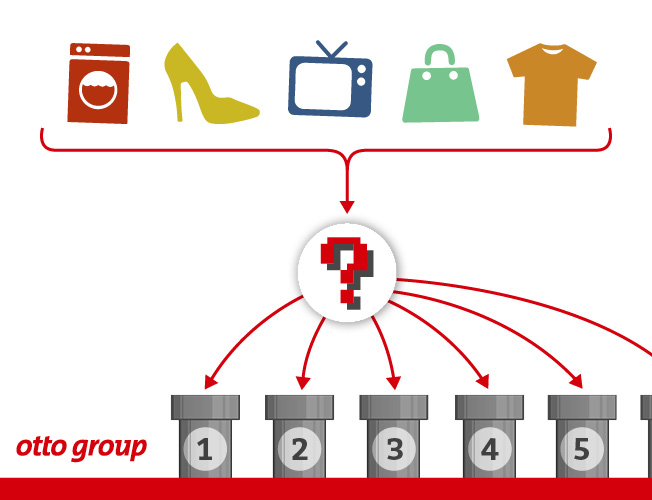
\includegraphics[width=0.6\textwidth,keepaspectratio]{otto}
	\caption{Otto product classification}
\end{figure}

\section{Data Analysis}
\subsection{Presenting the data}

Tha dataset provided by Otto has 61878 different products. Each sample is described by 93 categorical features. Values of the target variable can be one out of the 9 classes that the group identified. 

\begin{figure}[H]
	\centering
	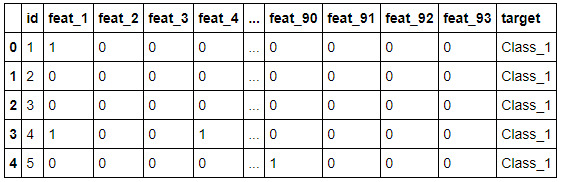
\includegraphics[width=0.6\textwidth,keepaspectratio]{data}
	\caption{Data presentation (61878 samples * 93 features * 9 classes)}
\end{figure}

\subsection{Exploratory Data Analysis}

Before tackling the classification problem, a good understanding of our data is needed. Thus, we will started by providing some statistics and features caracteristics .

\subsubsection{Features Distributions}

We plotted the distribution of all 93 features to see how they differ across products. The first thing to notice in the figures below is the dominance of  level 0 for all 93 fetures. Except for 2 or 3 features, the 75th percentile of the features distribution is 0. Since we have no idea about the sens of features in our data, we won't be able to figure out what a zero value means. Is might be either a missing value or a categorical level in itself. 

\begin{figure}[H]
	\centering
	\begin{subfigure}{0.22\textwidth}
		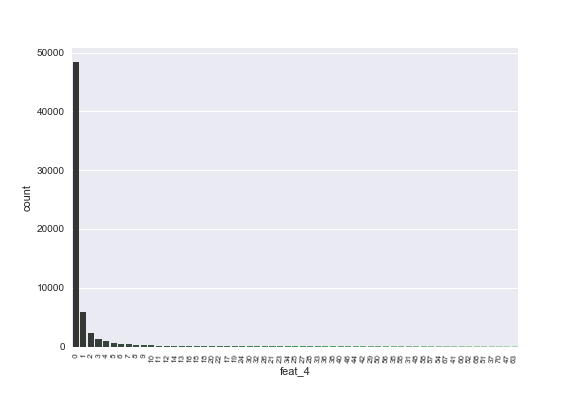
\includegraphics[width=\textwidth]{feat_4}
		\caption{Feature 4}
	\end{subfigure}
	\begin{subfigure}{0.22\textwidth}
		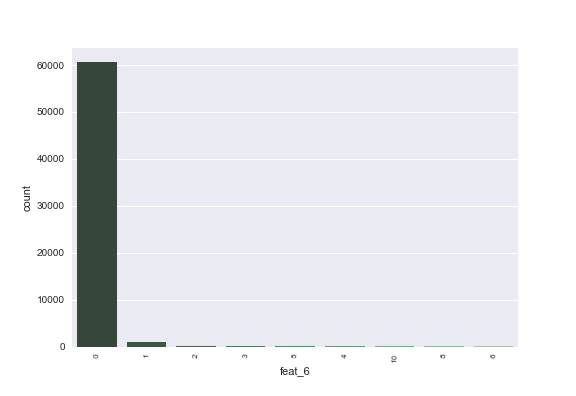
\includegraphics[width=\textwidth]{feat_6}
		\caption{Feature 6}
	\end{subfigure}
	\begin{subfigure}{0.22\textwidth}
		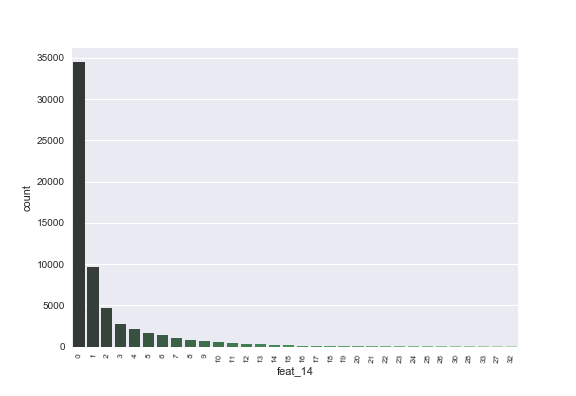
\includegraphics[width=\textwidth]{feat_14}
		\caption{Feature 14}
	\end{subfigure}	
	\begin{subfigure}{0.22\textwidth}
		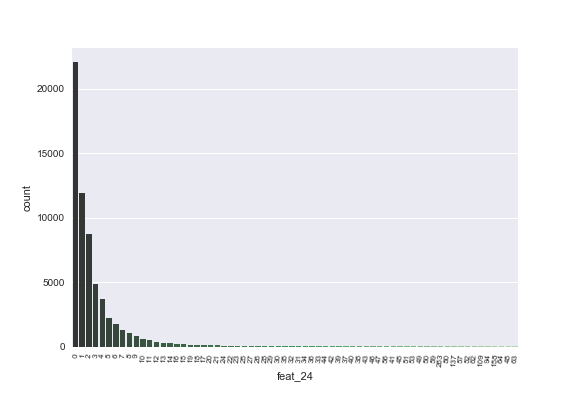
\includegraphics[width=\textwidth]{feat_24}
		\caption{Feature 24}
	\end{subfigure}	
	\caption{Some features distributions}
	\end{figure}


\subsubsection{Feature Correlation}

In figure \ref{correlation}, we show the correlation of the 93 features. As one may notice, a relatively high correlatio exis between a subset of features. For instance, top 10 highest correlation coefficients are shown in  figure \ref{top10}. Features like feat$_39$ and feat$_45$ are positively and highly correlated, with a coefficient of 0.82. Thus, we may think of a way to reduce dimensionality of the feature space, albeit no significant information loss occurs.

\begin{figure}[H]
	\centering
	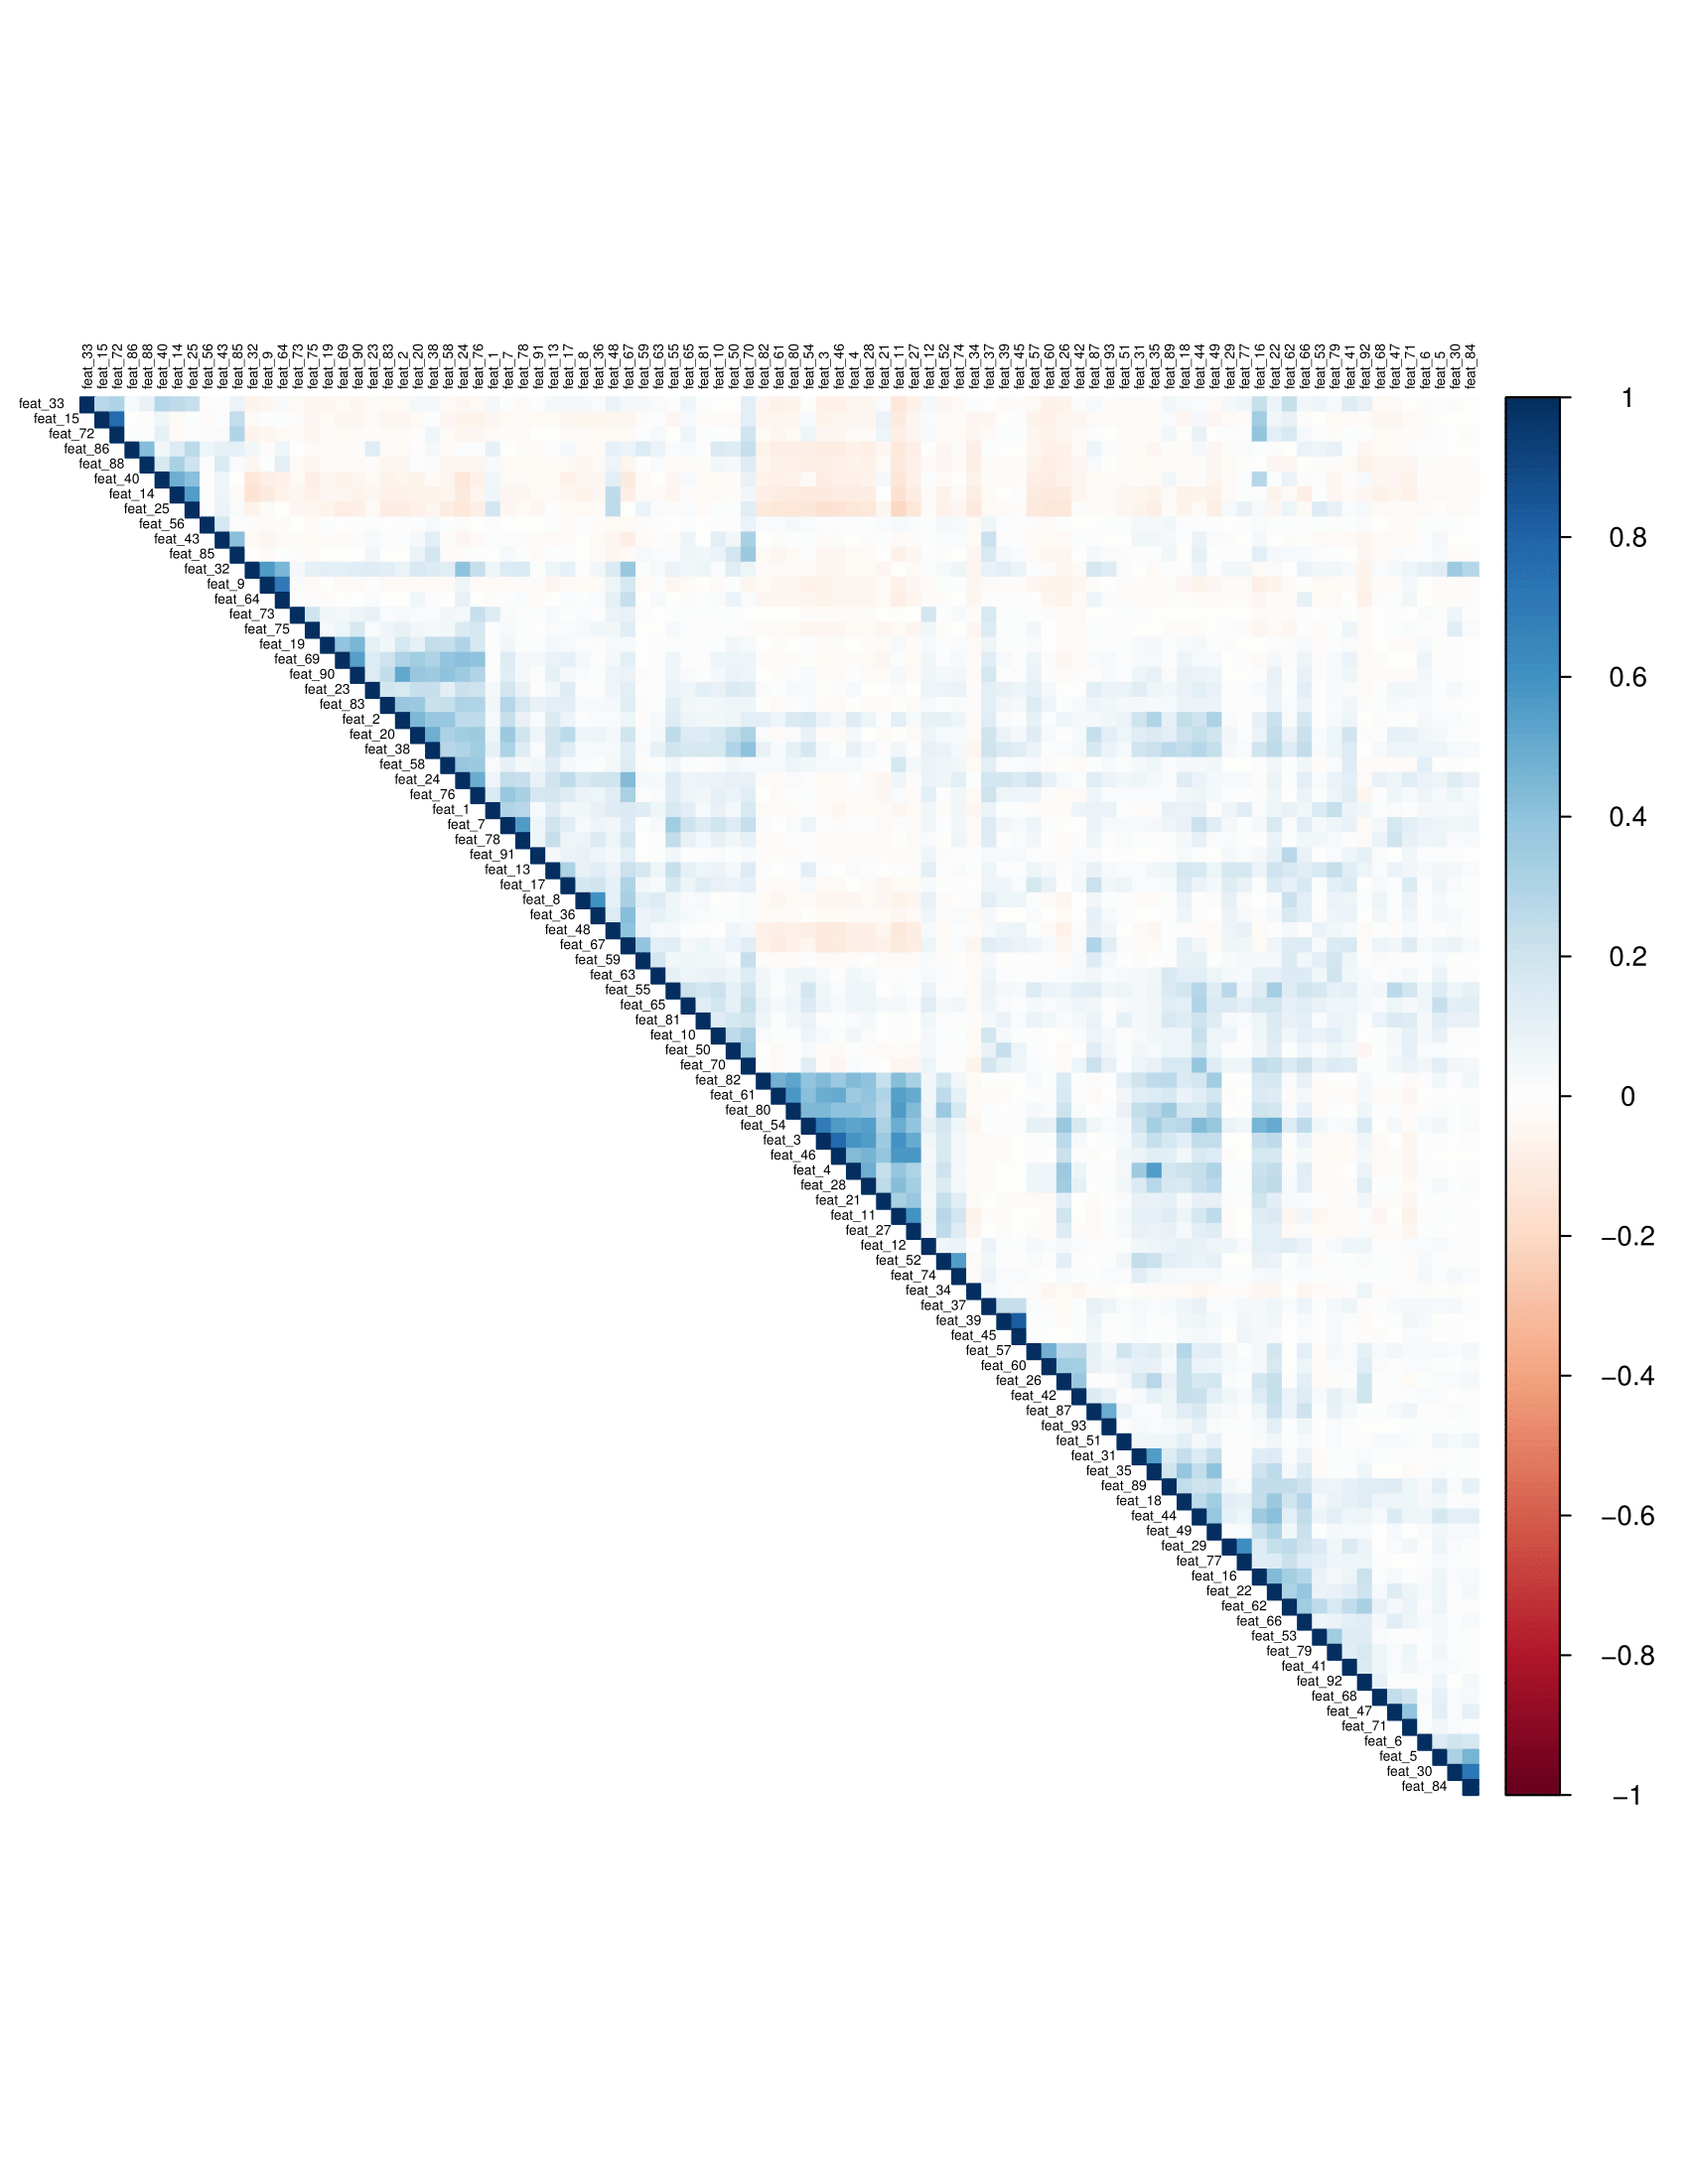
\includegraphics[width=0.8\textwidth,keepaspectratio]{corr_Otto}
	\caption{Correlation between features}
	\label{correlation}
\end{figure}

\begin{figure}[H]
	\centering
	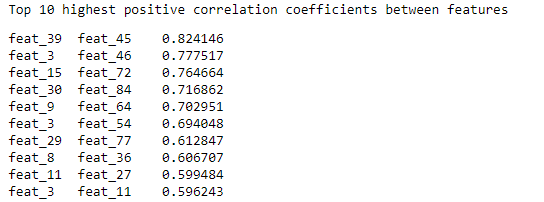
\includegraphics[width=0.7\textwidth,keepaspectratio]{top10_corr}
	\caption{Top 10 highest correlation coefficients}
	\label{top10}
\end{figure}

\subsubsection{Class Distribution}

In figures \ref{target} and \ref{class_dist} we show the distribution of the target variable and the proportion of each class in the data, respectively.  We clearly see that classes are very imbalanced, indicating that we should be careful later on when we move to classification.

\begin{figure}[H]
	\centering
	\begin{subfigure}{0.4\textwidth}
		\centering
		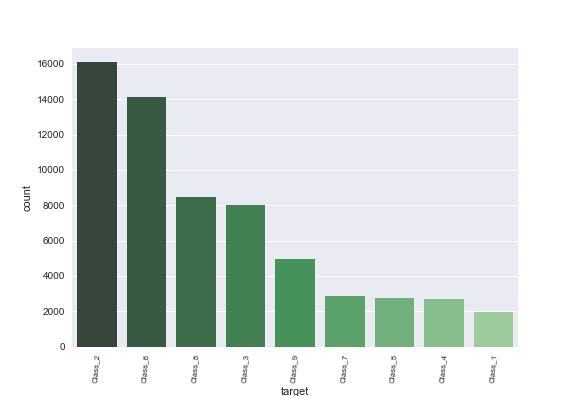
\includegraphics[width=0.95\textwidth]{target}
		\caption{Class distribution in Otto dataset}
		\label{target}
	\end{subfigure}
	\begin{subfigure}{0.4\textwidth}
		\centering
		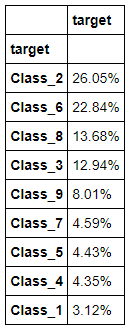
\includegraphics[width=0.3\textwidth]{class_dist}
		\caption{Class proportions}
		\label{class_dist}
	\end{subfigure}
\caption{Classes distribution}
\end{figure}


\section{Predictive Modeling}

In order to predict the class for each product, we tried several Scikit-Learn classification algorithms and compared their performances. Since it's a multiclass classification problem, we used a One-Vs-Rest classification schema  using the following models:
\begin{itemize}
\item Linear Support Vector Machines
\item Random Forests
\item Logistic Regression
\item MLP Classifier
\item Gaussian Naive Bayes
\end{itemize}

Since we are facing a class-imbalance problem, it is not wise to use simple accuracy to evaluate the model. Instead, we used the ROC AUC as a performance evaluation metric for our classifiers. Quoting Scikit-Learn documentation: "ROC curves typically feature true positive rate on the Y axis, and false positive rate on the X axis. This means that the top left corner of the plot is the “ideal” point - a false positive rate of zero, and a true positive rate of one. This is not very realistic, but it does mean that a larger area under the curve (AUC) is usually better. Although ROC curves are typically used in binary classification to study the output of a classifier, we may extend ROC curve and ROC area to multi-class or multi-label classification, but it is necessary to binarize the output first. One ROC curve can be drawn per label, but we can also draw a ROC curve by considering each element of the label indicator matrix as a binary prediction (micro-averaging).

Another evaluation measure for multi-class classification is macro-averaging, which gives equal weight to the classification of each label.

The “steepness” of ROC curves is also important, since it is ideal to maximize the true positive rate while minimizing the false positive rate".

We also checked the performace of some models when they are applied to PCA-transformed data. 

Finally, we used bagging of different classiers and evaluated its performance. Voting is one of the simplest ways of combining the predictions from multiple machine learning algorithms.It works by first creating two or more standalone models from the training dataset. A Voting Classifier can then be used to wrap the models and average the predictions of the sub-models when asked to make predictions for new data.

\subsection{Results}
In the figure below, we show the ROC curves resulting from the predictions of the models used. 

\begin{figure}[H]
	\centering
	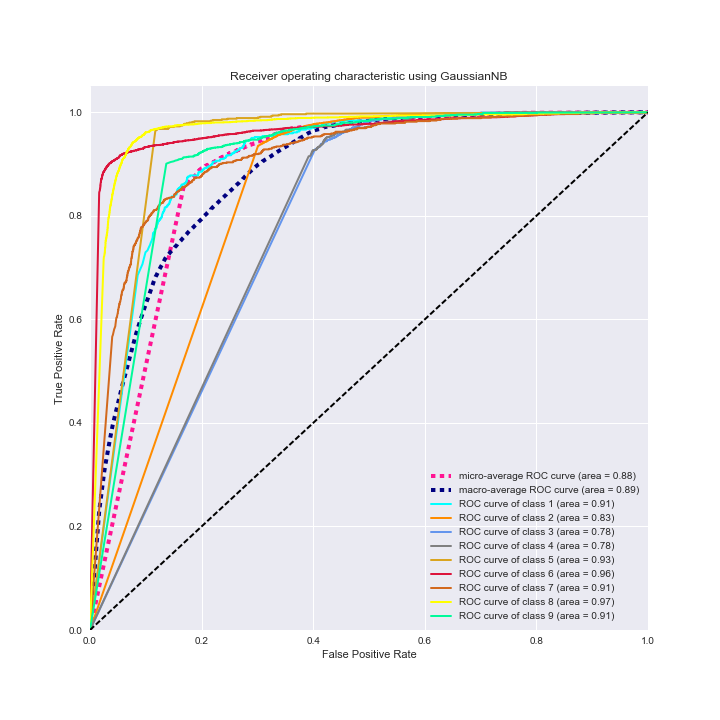
\includegraphics[width=0.9\textwidth,keepaspectratio]{ROC_OvR_GaussianNB}
	\caption{ROC for GaussianNB}
\end{figure}

\begin{figure}[H]
	\centering
	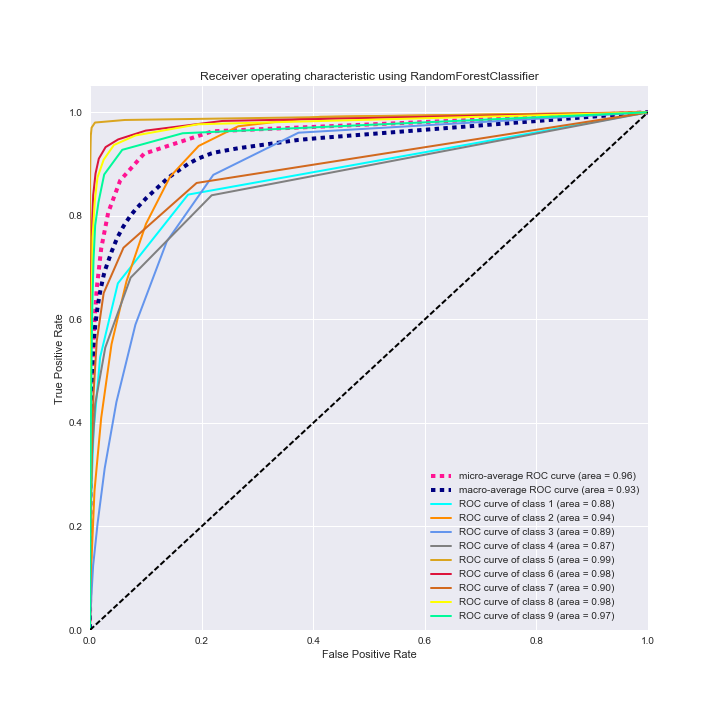
\includegraphics[width=0.9\textwidth,keepaspectratio]{ROC_OvR_RandomForestClassifier}
	\caption{ROC for Random Forests}
\end{figure}

\begin{figure}[H]
	\centering
	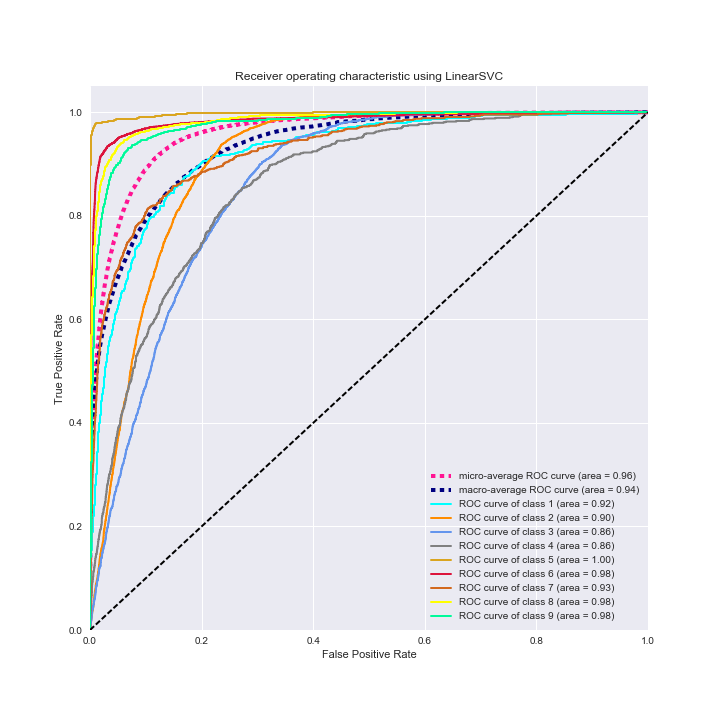
\includegraphics[width=0.9\textwidth,keepaspectratio]{ROC_OvR_LinearSVC}
	\caption{ROC for Linear SVC}
\end{figure}

\begin{figure}[H]
	\centering
	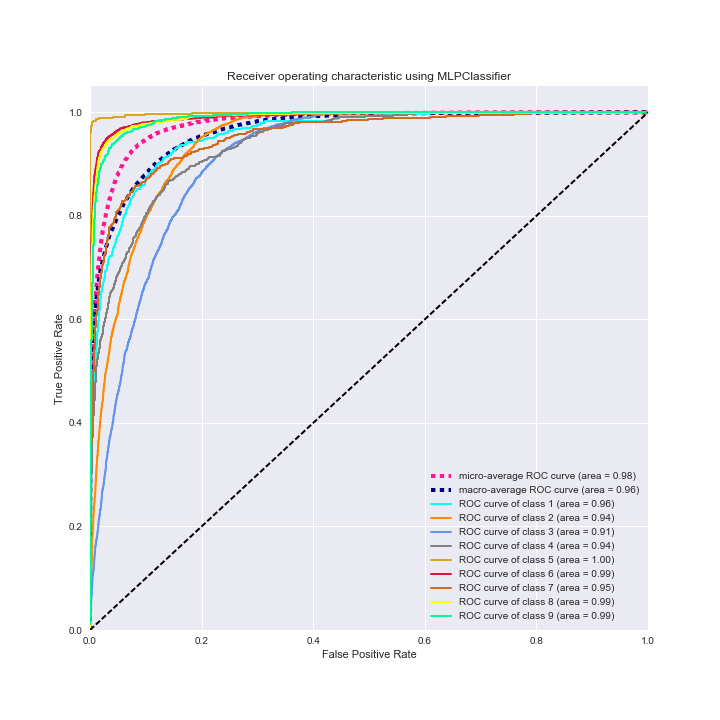
\includegraphics[width=0.9\textwidth,keepaspectratio]{ROC_OvR_MLPClassifier}
	\caption{ROC for MLP}
\end{figure}

Clearly, the GaussianNB does not perform well on our data. However, Random Forests, SVM and MLP seem to have better AUCs. Also, their corresponding curves are steep, indication a good trade-off between True positives and False positives. We also notice that the curves differ from one class to another, reflecting the degree of difficulty to distinguish it from the other classes. 

\begin{figure}[H]
	\centering
	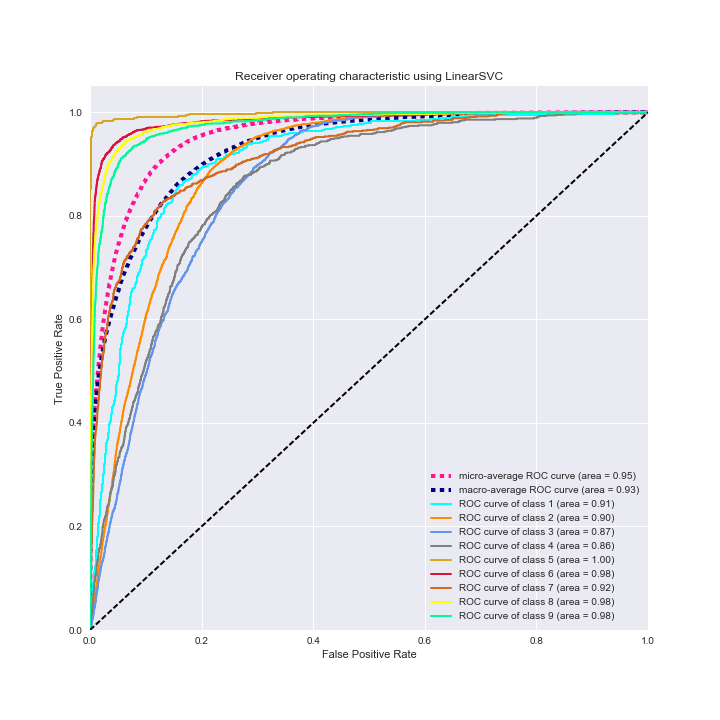
\includegraphics[width=0.9\textwidth,keepaspectratio]{ROC_OvR_LinearSVC_using_PCA}
	\caption{ROC for SVM using class weights for the PCA-transformed data}
\end{figure}

We can notice that using the PCA-transformed feature space, we don't loose too much information when we use LinearSVC with balanced class weights as a classifier. Thus, for the sake of computation time optimization, one would prefer to use the reduced data rather than the initial one.

\begin{figure}[H]
	\centering
	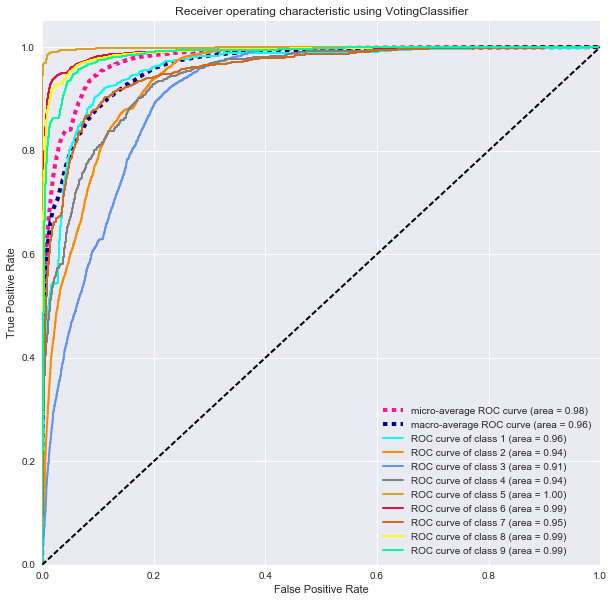
\includegraphics[width=0.9\textwidth,keepaspectratio]{ROC_OvR_Voting}
	\caption{ROC for the Voting Classifier}
\end{figure}

As for the Voting Classifier, overall performance is now clearly enhanced, which is already expected. 

\section{Conclusion}
This is a conclusion

%%%%%%%%%%%%%%%%%%%%%%%%%%%%%%%%%%%%%%%%%%%%%%%%%%%%%%%%%%%%%
\bibliographystyle{babplain}
\parskip=-1em
%\emptypage{\bibliography{bibliographie}}
\let\section\oldsection % pour éviter que le résumé soient visibles dans le sommaire comme une section
%\include{Resume}
\end{document}
